%%%%%%%%%%%%%%%%%%%%%%%%%%%%%%%%%%%%%%%%%%%%%%%%%%%%%%%%%%%%%%%%%%% 
%                                                                 %
%                           INLEIDING                             %
%                                                                 %
%%%%%%%%%%%%%%%%%%%%%%%%%%%%%%%%%%%%%%%%%%%%%%%%%%%%%%%%%%%%%%%%%%% 


\chapter{Besluit}  

In deze thesis hebben we onderzocht of het mogelijk is een interface te ontwerpen die het mogelijk maakt kristallen te visualiseren in het open source tekenprogramma Blender. Dit onderzoek hebben we onderverdeeld in drie algemene stappen: een studie van de \textit{state of the art}, het ontwerpen van het programma en ten slotte het uitvoeren van testen.
\par
In de eerste van deze stappen hebben we een stap gezet in de wereld van kristallografie, om zo een beter zicht te krijgen over hoe kristallen worden opgebouwd. Zo hebben we kennis gemaakt met de eenheidscel van een kristal. Dit is een driedimensionaal rooster waarbinnen de volledige structuur van een kristal zich bevindt. Ongeacht de grootte van een kristal, zal dit steeds bestaan uit een aaneenschakeling van deze eenheidscellen. 
\par
Een eenheidscel wordt steeds beschreven aan de hand van zes getallen die de roosterparameters worden genoemd. Drie van deze beschrijven de lengtes van de ribbes, terwijl de overige drie de hoeken ertussen bepalen. De vorm van zo een eenheidscel in echter niet willekeurig, Bravais, een Franse natuurkundige, was in staat op basis van de vorm en symmetrie van kristallen 14 verschillende manieren gevonden waarmee kristalroosters kunnen worden opgebouwd, welke we de Bravaisroosters noemen.
\par
Ook de posities van de atomen binnen een kristal zijn bepaald volgens enkele regels, dit wordt de inwendige symmetrie van een kristal genoemd en geeft ons een totaal van 230 verschillende manieren waarop deeltjes in een eenheidscel kunnen worden geordend.
\par
Het CIF-formaat is een digitaal formaat waarin de data van een kristal wordt opgeslagen. Doordat dit formaat in ASCII-codering is geschreven, is dit leesbaar door zowel mens als computer. Dit maakt het CIF-formaat een erg geschikt formaat om als invoer te gebruiken voor onze interface. Een CIF-bestand bestaat steeds uit één of meerdere datablokken die een aantal parameters bevat. Deze parameters worden gevolgd door de waarde van deze parameters en bevatten alle informatie die nodig is om een kristal te tekenen. Het CIF-formaat geeft echter niet alle elementen die in de eenheidscel voorkomen maar beperkt zich tot de combinatie van elementen en inwendige symmetrieoperaties waarmee de positie van elk element kan berekend worden. Voor deze berekening hebben we gebruik gemaakt van OpenBabel. OpenBabel maakt met de gegeven data een nieuw CIF-bestand aan dat exact hetzelfde kristal beschrijft, maar waar in plaats van symmetrieoperaties, de lijst van alle atomen in de eenheidscel wordt gegeven. 
\par
Vooraleer we dit CIF-bestand konden visualiseren moesten we op zoek gegaan naar een manier om de data uit het CIF-formaat in meer bruikbare datastructuren op de slaan. Dit hebben we gedaan door het CIF-bestand te parsen met de CifFile module van PyCIFRW en de verkregen data op te slaan in verschillende klassen die we hebben aangemaakt. 
\par
Om objecten te tekenen in Blender moesten we gebruik maken van de bpy module van de Blender API. Naast het tekenen van atomen wilden we ook de mogelijkheid hebben tot het tekenen van een omkadering van de eenheidscel en eventuele bindingen tussen atomen. Eerst zal de omkadering getekend worden door bollen te tekenen op de hoekpunten van de cel en tussen deze cilinders te tekenen. 
\par
Voor het tekenen van de atomen hebben we twee externe dictionaries gemaakt die voor elk bestaand element de straal en de kleur van het atoom bijhouden. Vervolgens wordt de lijst met atomen doorlopen en bepalen we voor elk atoom de positie, straal en kleur. Ten slotte berekenen we de afstand tussen alle atomen, en tekenen we een binding tussen twee atomen wanneer hun onderlinge afstand minder is dan een door de gebruiker bepaalde waarde. 
\par
Ten slotte hebben we gekozen een Blender add-on te maken van ons programma, waardoor het eenvoudig kan gebruikt worden in de Blender omgeving. Door het programma als een add-on aan te bieden kan een gebruiker met behulp van een grafische interface kristallen tekenen in plaats van het programma manueel uit te voeren in Blender. 
\par
Het eerste deel van het ontwerpen van de add-on, te zien op Figuur[6.2], was het maken van operatoren die de functionaliteiten van het programma aansturen. Het tweede deel van het ontwerpen van de add-on was het ontwerpen van een paneel. Met een paneel kan de opmaak en structuur van de add-on gepersonaliseerd worden. 
\par  
\begin{figure}[H]
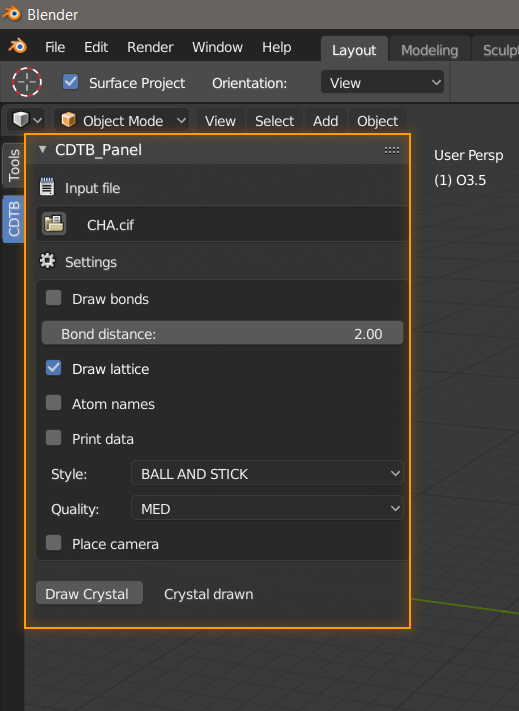
\includegraphics[scale=0.5]{paneel.png}
\caption{De add-on zoals te zien in Blender}
\end{figure}

We hebben ook enkele testen uitgevoerd en nadien de resultaten vergeleken met het kristalvisualisatieprogramma VESTA. Op vlak van snelheid deed ons programma er ongeveer een halve seconde over om een klein kristal met bindingen te tekenen, terwijl dit voor een groot kristal meer dan twee minuten duurde. Het tekenen van het kleine kristal deed VESTA 17 maal sneller en het grote kristal tekende VESTA zelfs 400 maal sneller dan ons programma. Op vlak van gebruiksvriendelijkheid hing het vooral af van de toepassing, hoewel VESTA dankzij het grote aantal aan features het meest geschikt was voor wetenschappelijk gebruik, was het minder eenvoudig in omgang en was het kristalmodel minder interactief. 
\par
Ons programma overtrefte VESTA wel op vlak van uitbreidbaarheid. Dit was omdat het niet mogelijk is als gebruiker features toe te voegen aan VESTA, terwijl ons programma zo geschreven is dat het toevoegen van features relatief eenvoudig is. 
\par 
Een nadeel van ons programma is dat het gemaakt is voor de allernieuwste versie van Blender, die eigenlijk nog in beta is. Hierdoor is het moeilijker informatie te vinden over de functionaliteiten van de Blender API, ondanks de duidelijke documentatie.
\par
Er is een functionaliteit in ons programma die niet werkt door een probleem in de CifFile module van PyCIFRW. Dit probleem leidt ertoe dat er geen lange padnamen kunnen worden meegegeven met de inleesfunctie waardoor enkel bestanden in de werkmap kunnen worden ingelezen. Hierdoor is er steeds nood aan OpenBabel, terwijl het programma ook zonder zou moeten kunnen lopen.
\par
Door de uitbreidbaarheid van het programma en de mogelijkheden die de Blender API biedt, is \textit{The sky the limit}. Enkele features die zeker interessant zijn in de toekomst toe te voegen zijn:
\begin{itemize}
\item De gebruiker de mogelijkheid geven de grenzen te bepalen waarbinnen getekend moet worden
\item Een individuele bindingsafstand per element zodat foute bindingen vermeden kunnen worden
\item Het implementeren van modules uit de cctbx 
\end{itemize}
 